\documentclass[12pt, titlepage]{article}

\usepackage[T1]{fontenc}
\usepackage[margin=1in]{geometry}
\usepackage{indentfirst}
\usepackage{booktabs}
\usepackage{graphicx}

\title{The BigDuck\\Programming Language Proposal}
\author{Jair Antonio Bautista Loranca}

\begin{document}
\maketitle
\tableofcontents

\section{Objective}
\paragraph{} This document is to describe the general characteristics for the
BigDuck programming language. BigDuck is language aimed for the developement of
mathematical models commonly used in Machine-Learning and Data Science.

\paragraph{} Therefore this language will include integer and floating point
arithmetic, vector and matrix operations, and some basic utilities for reading
and writing \texttt{.csv} files. All this with the purpose to make it easier
for the user to work within the Machine-Learning and Data Science fields.

\section{Language Requirements}
\subsection{Basic Elements}
\subsubsection{Identifiers}
\paragraph{} In this language identifiers can be build starting with any
alphabetic character followed by the any sequence of alphanumeric characters or
underscore characters, and terminated by any whitespace character. This being
identical to the common convention used in many popular programming languages
like C, Java, or Python.

\newpage

\subsubsection{Whitespace and comments}
\emph{Whitespace} charaters include spaces, tabs, newlines. The BigDuck
compiler ignores whitespace characters, however the usage of this is recommend 
and may be use to align text to improve readability.

\paragraph{} The token \texttt{\#|} indicates the start of a comment and
must be closed by the token \texttt{|\#} to end the comment. All the text
inside this tokens will be ignored by the compiler. Comments are just help
clarify or document programs.

\subsubsection{Reserved Keywords}
\begin{verbatim}
proc                return              if                  else
loop                break               skip                and
or                  not                 var                 int
float               bool                true                false
\end{verbatim}

\paragraph{} Most of these keywords are used in many programming languages so
they do not require explanation, however some some of them defer.

\paragraph{} \texttt{proc} is use to specify a procedure declaration. 

\paragraph{} \texttt{loop} is use instead of the usual \texttt{while},
\texttt{do while}, and \texttt{for} keywords. The rational is that all of these
can be rewritten into a for-loop, however the traditional for-loop reading
gets messed up when doing this, therefore the \texttt{loop} keyword was chosen
instead.

\paragraph{} \texttt{skip} is use instead of the usual \texttt{continue}. The
rational for this replacement is that it is more descriptive of the action
performed.

\subsubsection{Other notations}
\paragraph{} There are several tokens left out from this section, however these
will be mention within their syntactical or semantic context. This is to avoid 
redundancy on this document.

\subsection{Syntax Diagrams}

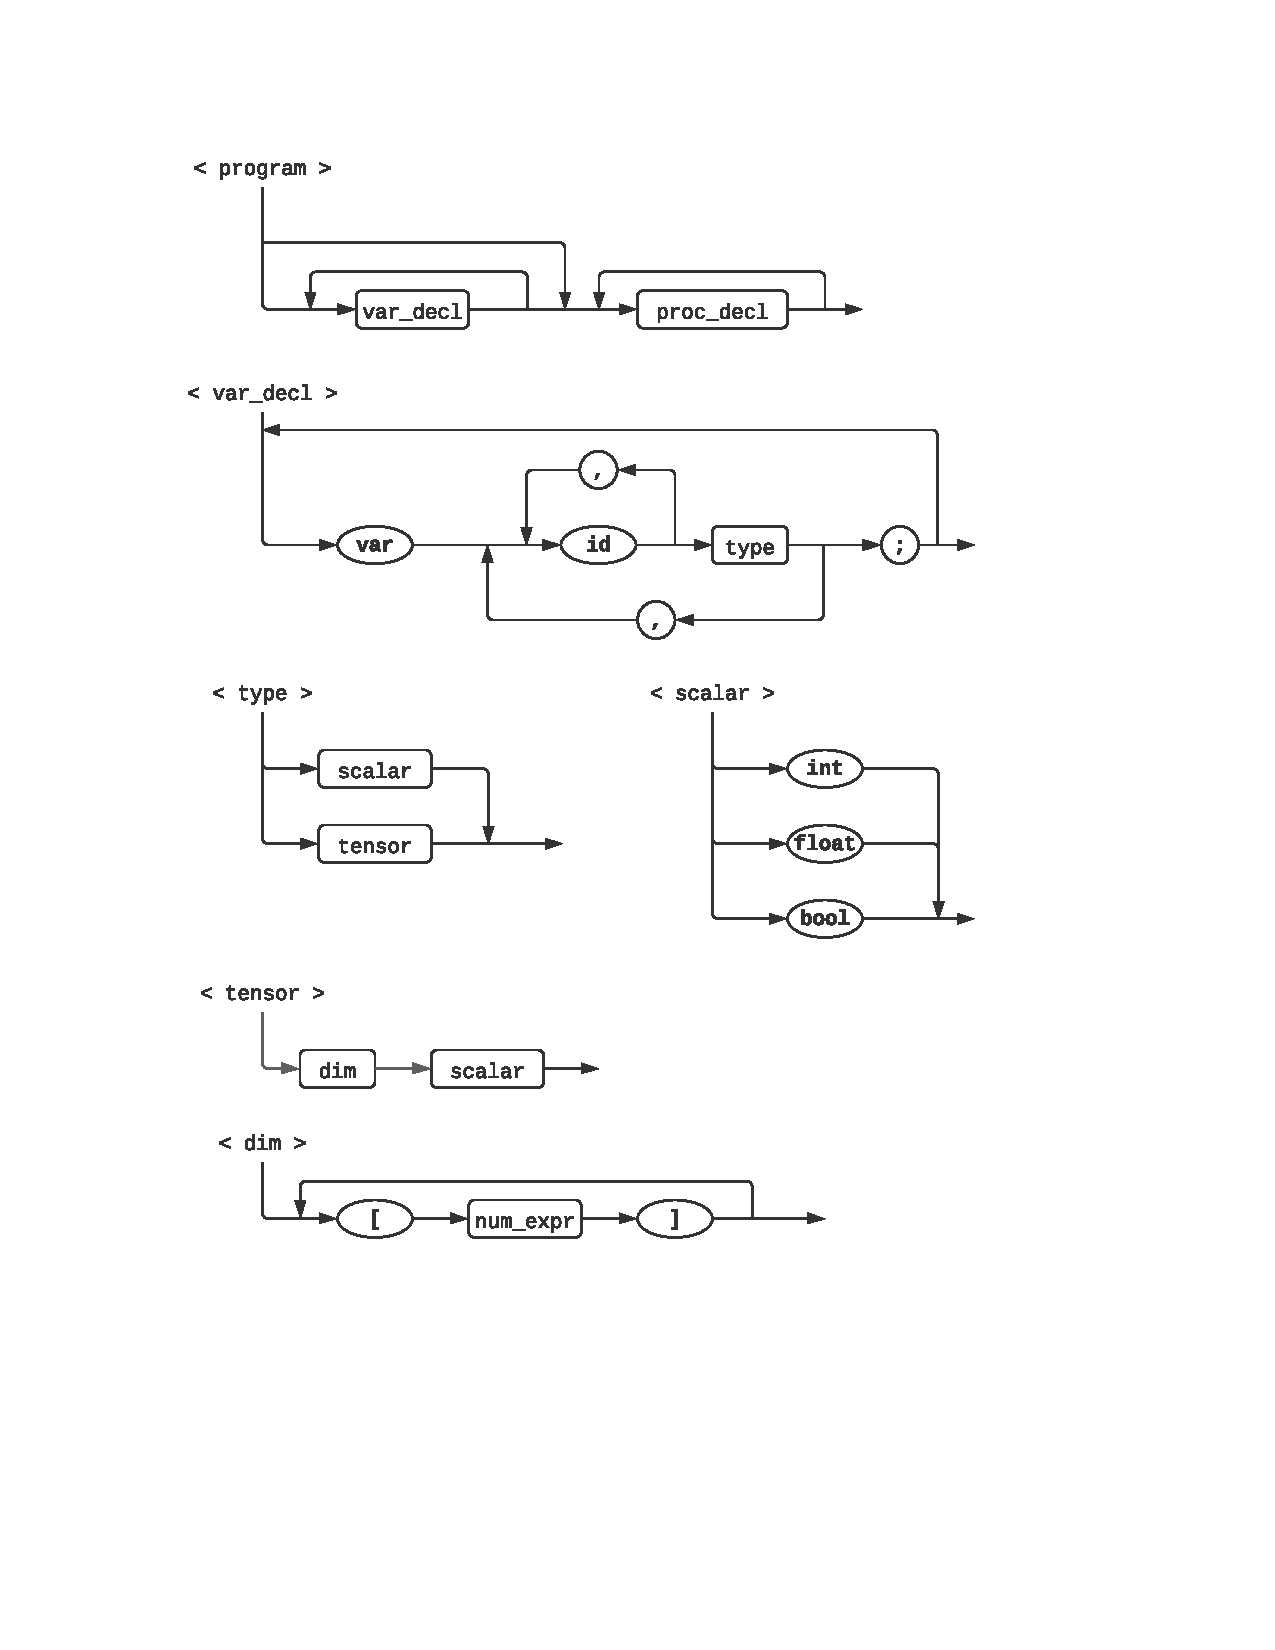
\includegraphics[trim={1in, 1in, 1in, 1in}, clip, scale=0.95]{d1}
\newpage
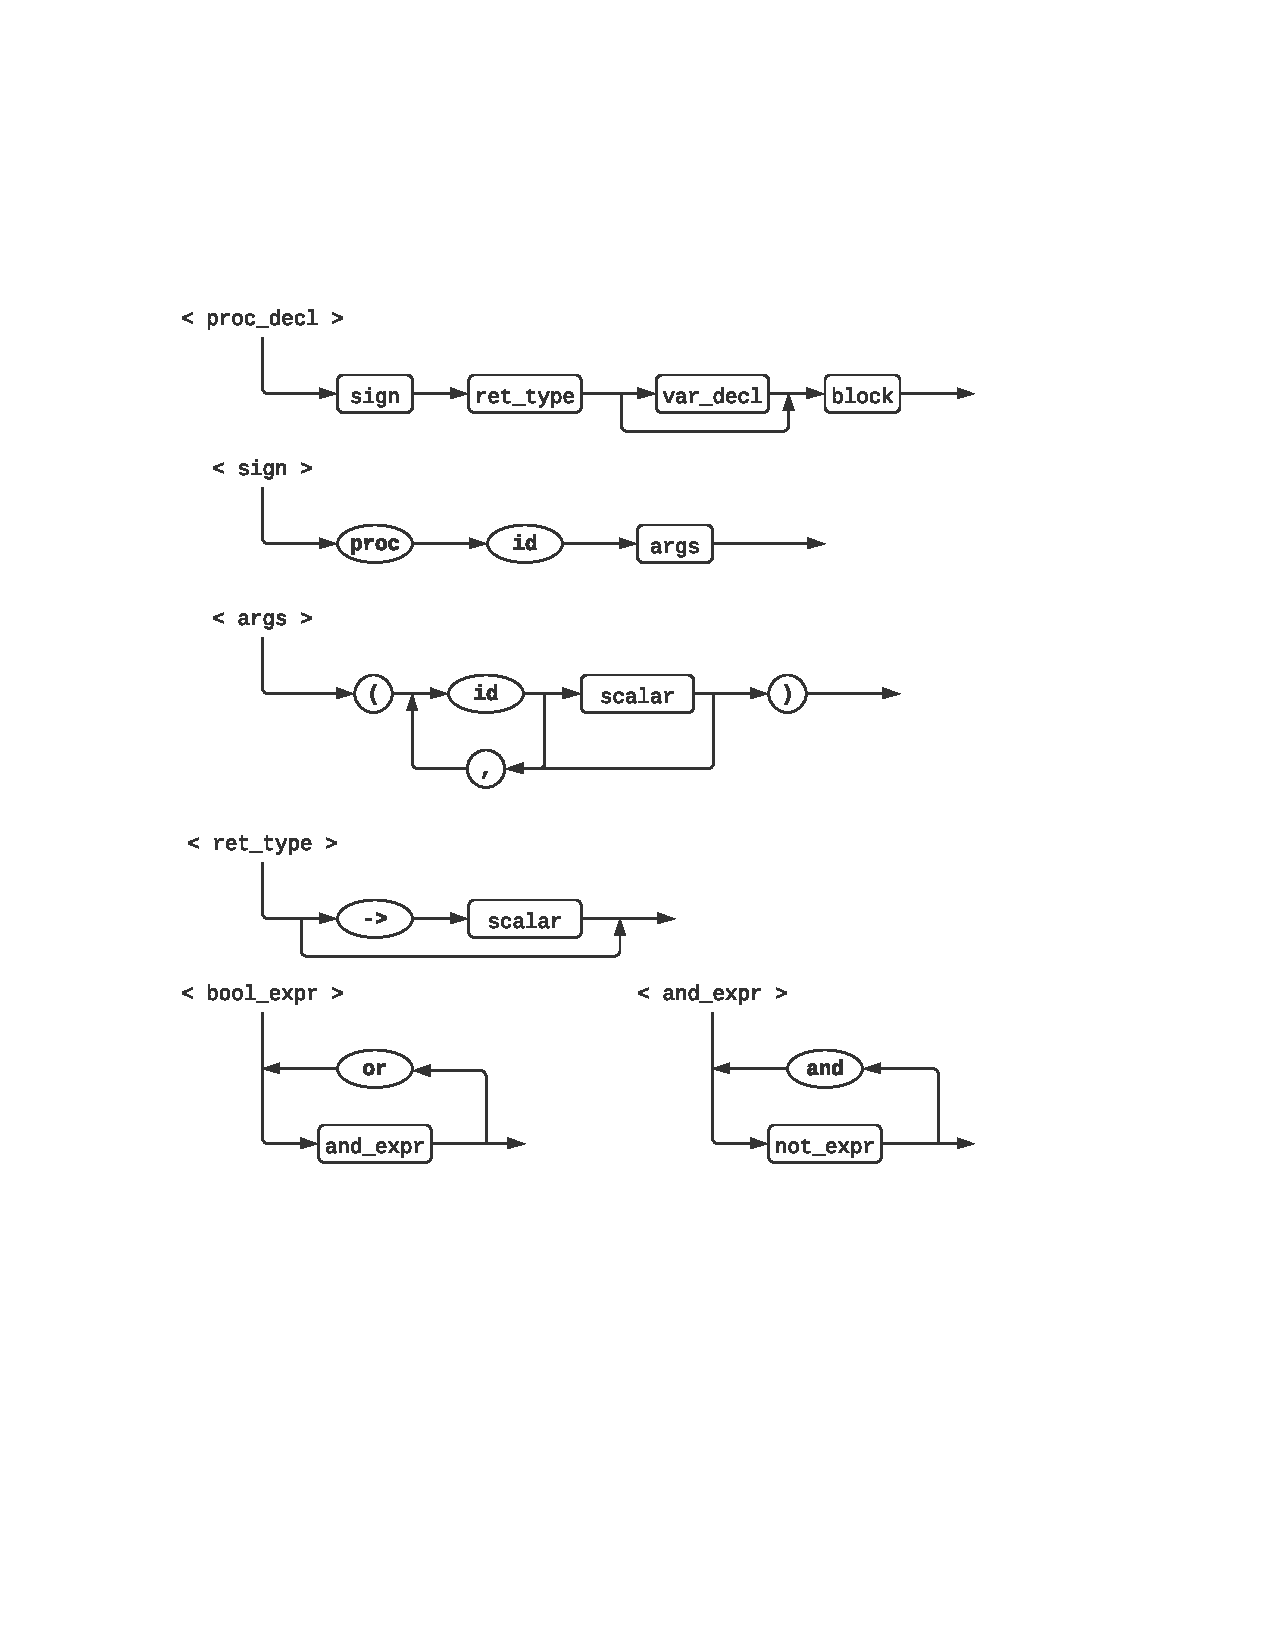
\includegraphics[trim={1in, 1in, 1in, 1in}, clip, scale=0.95]{d2}
\newpage
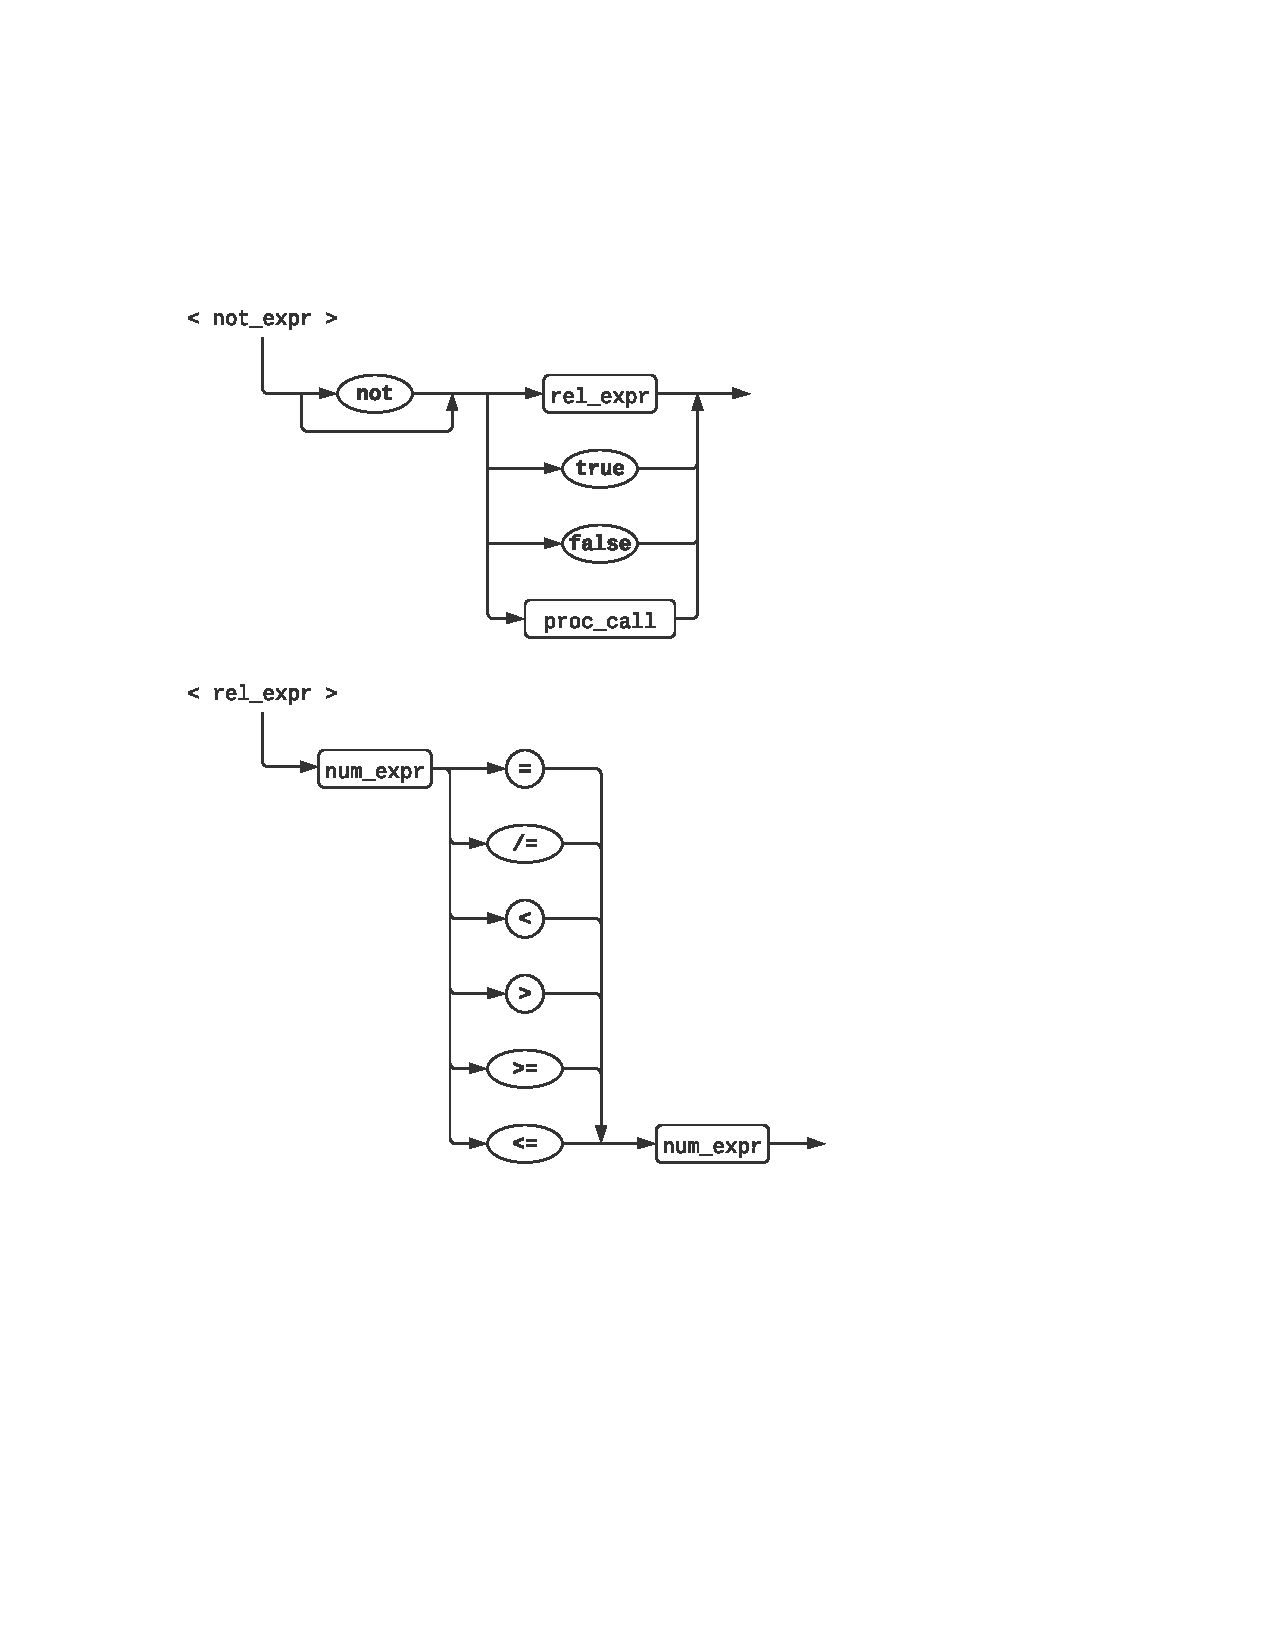
\includegraphics[trim={1in, 1in, 1in, 1in}, clip, scale=0.95]{d3}
\newpage
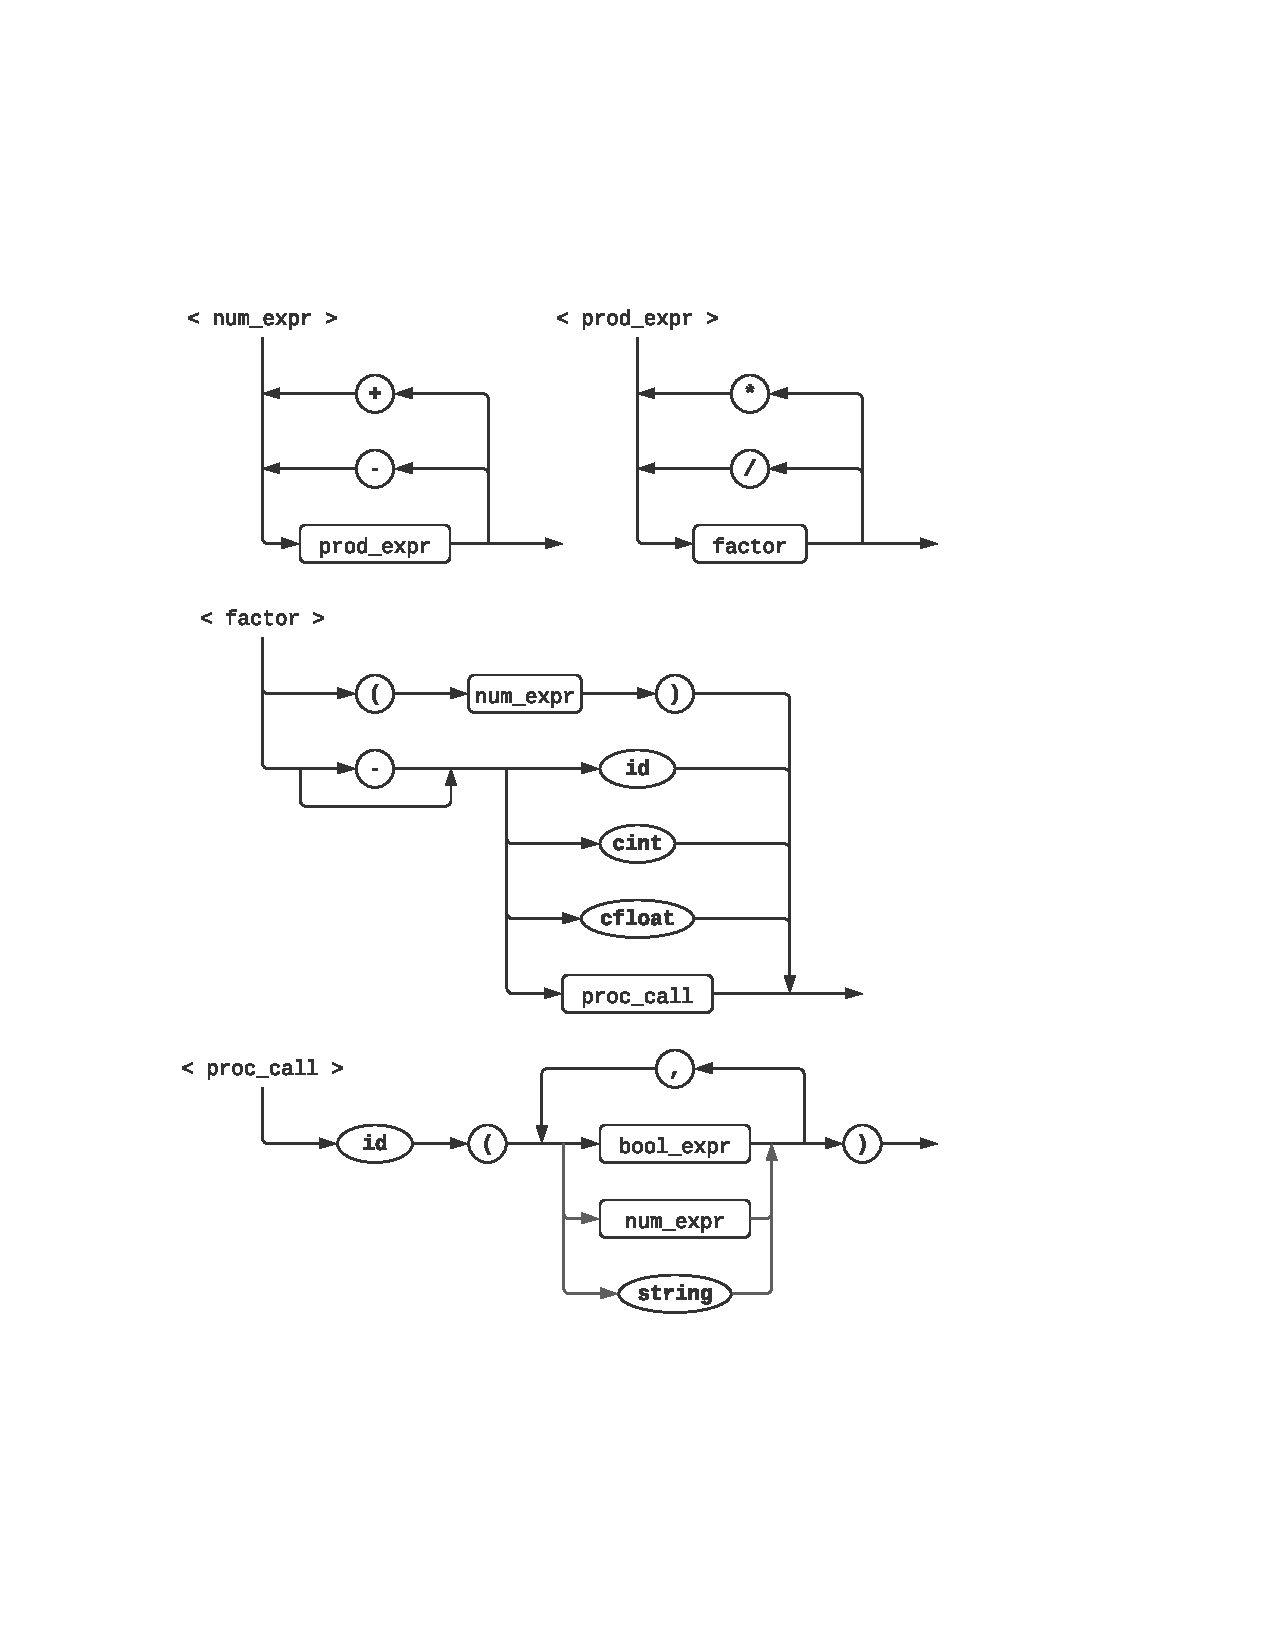
\includegraphics[trim={1in, 1in, 1in, 1in}, clip, scale=0.95]{d4}
\newpage
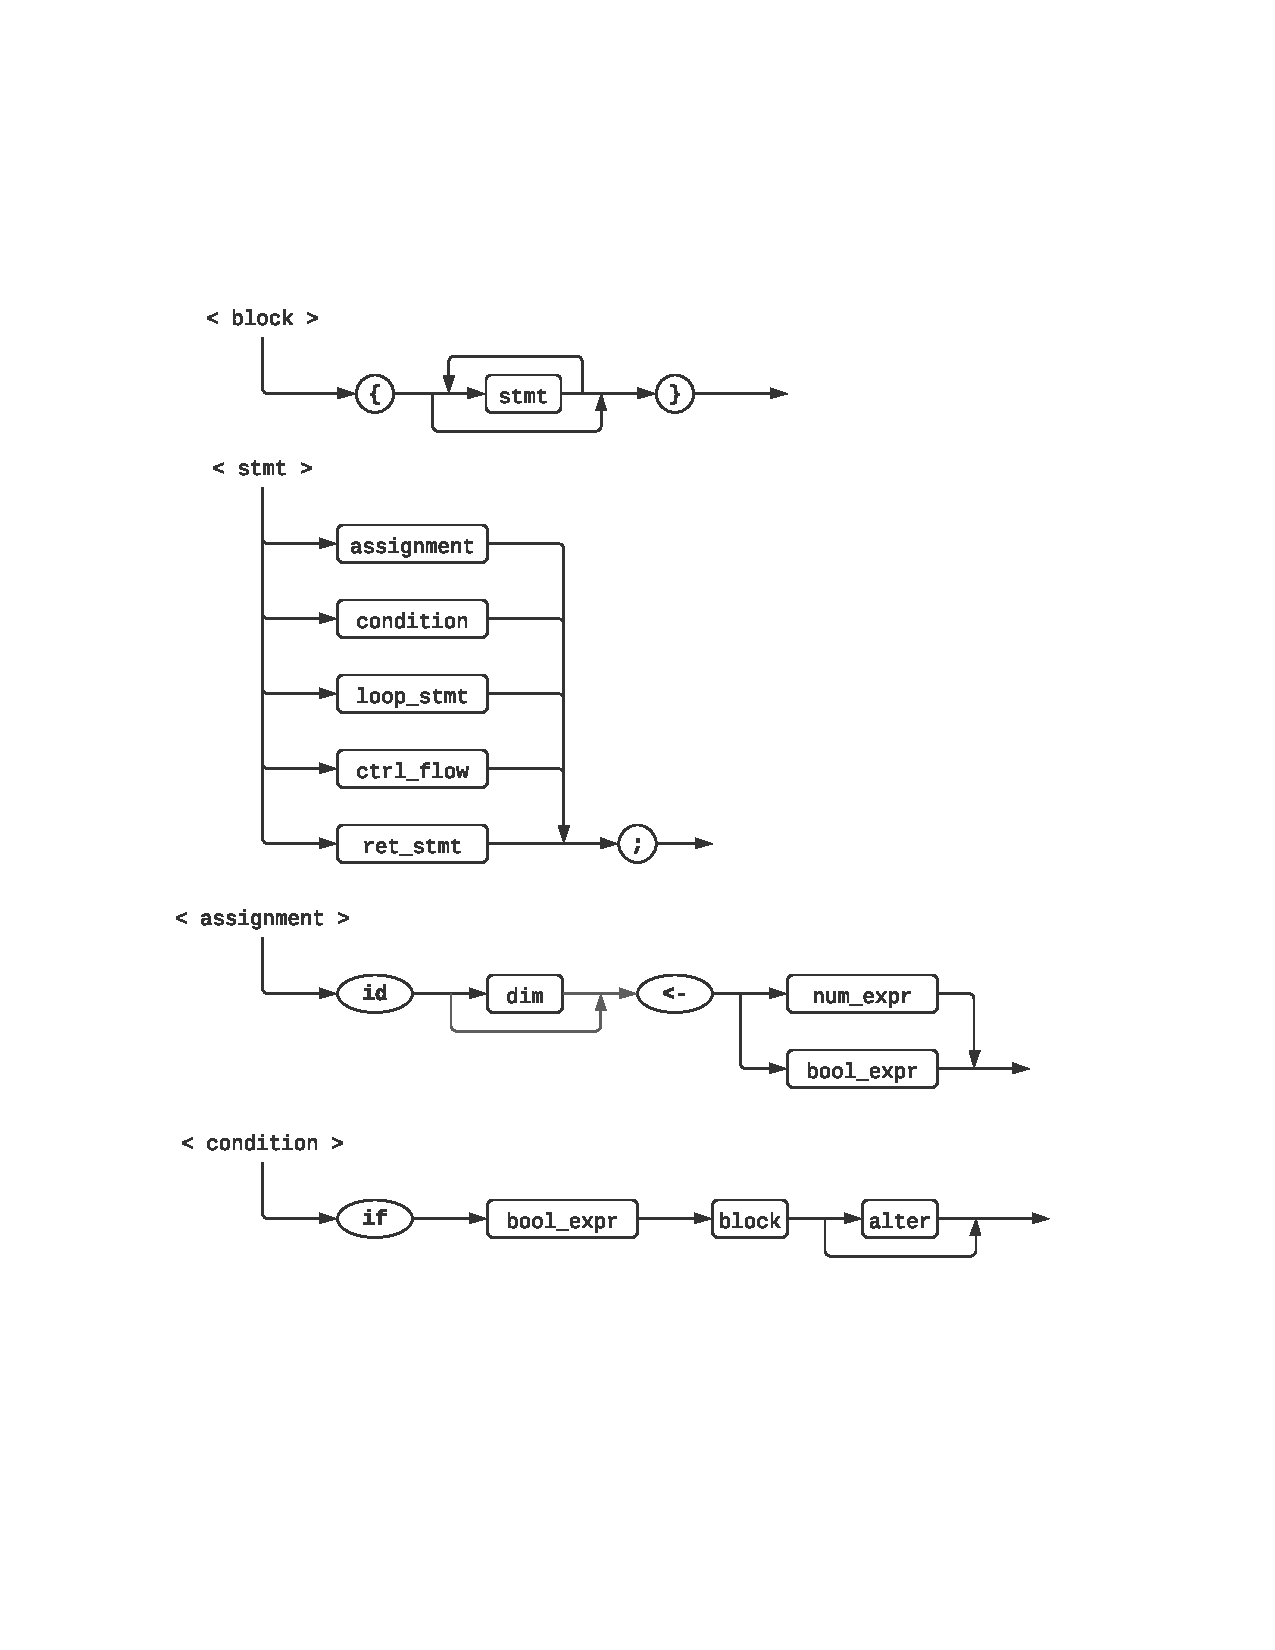
\includegraphics[trim={1in, 1in, 1in, 1in}, clip, scale=0.95]{d5}
\newpage
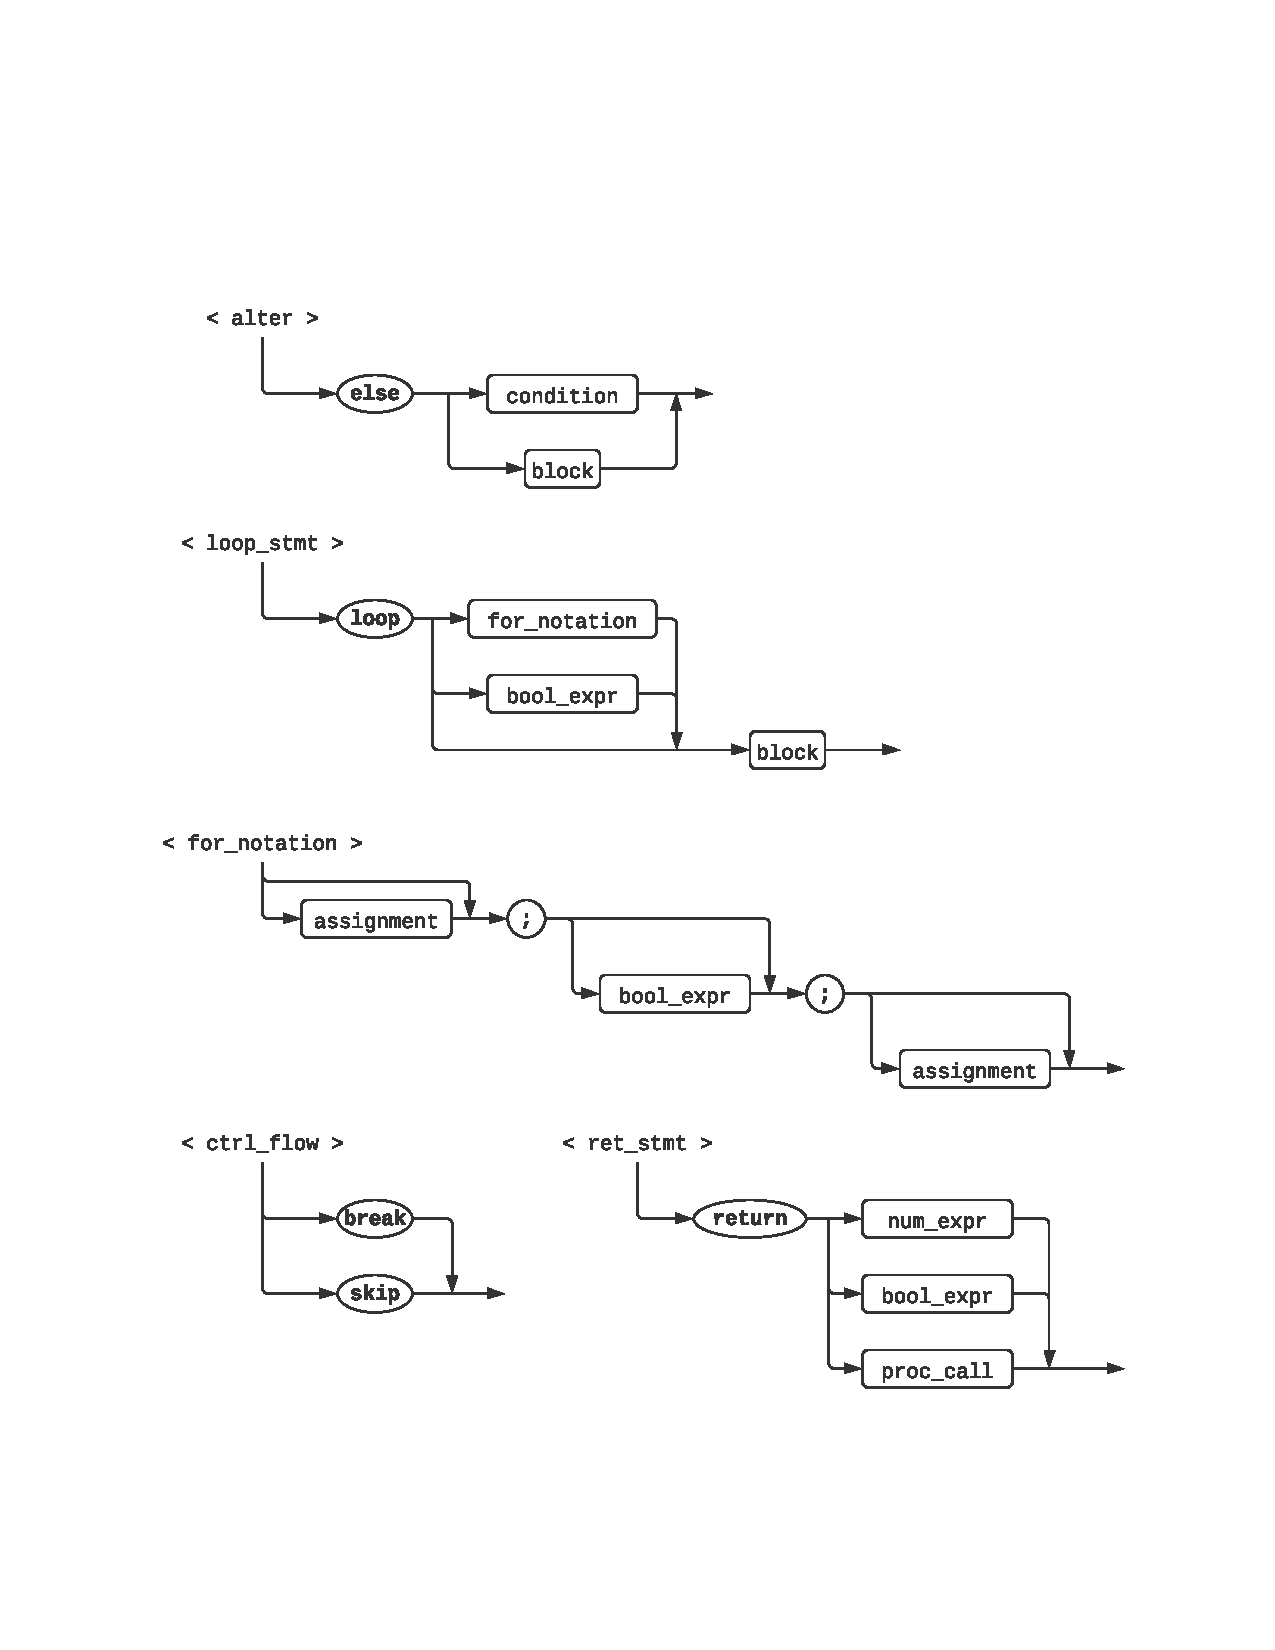
\includegraphics[trim={1in, 1in, 1in, 1in}, clip, scale=0.95]{d6}
\newpage

\subsection{Sematic Characteristics}\label{semantics}
\paragraph{} Following popular programming languages like C, Java, Go, etc,
BigDuck is a statically scoped language. Meaning that each variable exists
within their scope of definition. However there are only two scopes: global
scope and procedure scope. BigDuck is a statically typed language, meaning that 
variables can only contain values of the same type.

\paragraph{} Arguments to procedures are always passed by value, and all 
parameter expressions in a procedure call are evaluated first wether the
procedure needs the result of the evaluation or not. As opposed to lazy 
evaluation done in some functional languages like Haskell.

\paragraph{} There must be at least one procedure defined, the last procedure
on the program will be taken as the main procedure for the program.

\subsection{Built-in procedures}
\paragraph{IO operations}
\begin{verbatim}
#| Prints any object given |#
proc print(any)

#| Reads value from input|#
proc read(any) -> any

#| Opens csv file |#
proc open_csv(filename, sep string, header bool) -> [][]any

#| Writes object to a csv file |#
proc write_csv(filename string, any)
\end{verbatim}

\paragraph{Math operations}
\begin{verbatim}
#| Returns the arccosine for a given angle |#
proc acos(x float) -> float

#| Returns the arcsine for a given angle |#
proc asin(x float) -> float

#| Returns the arctangent for a given angle |#
proc atan(x float) -> float

#| Returns the arctangent for the quotient y / x |#
proc atan2(y, x float) -> float

#| Returns the cosine for a given angle |#
proc cos(x float) -> float

#| Returns the sine for a given angle |#
proc sin(x float) -> float

#| Returns the tangent for a given angle |#
proc tan(x float) -> float

#| Returns the hyperbolic cosine for a given angle |#
proc cosh(x float) -> float

#| Returns the hyperbolic sine for a given angle |#
proc sinh(x float) -> float

#| Returns the hyperbolic tangent for a given angle |#
proc tanh(x float) -> float

#| Returns e to power of the given exponent |#
proc exp(x float) -> float

#| Returns the natural logarithm for a given number |#
proc ln(x float) -> float

#| Returns the logarithm base b for a given number x |#
proc log(x, b float) -> float

#| Returns the mod base b for a given number x |#
proc mod(x, b float) -> float

#| Returns the remainder of the quotient x / b |#
proc rem(x, b float) -> float

#| Returns x to the power of the given exponent y |#
proc pow(x, y float) -> float

#| Returns the squared root for a given number |#
proc sqrt(x, y float) -> float

#| Returns the absolute value for a given number |#
proc abs(x, y float) -> float

#| Returns the ceiling for a given number |#
proc ceil(x float) -> float

#| Returns the floot for a given number |#
proc floor(x float) -> float
\end{verbatim}

\paragraph{Vector operations}
\begin{verbatim}
#| Returns the magnitude for a given vector |#
proc mag(v1 []float) -> float

#| Returns the euclidean distance for two given vectors |#
proc dist(v1, v2 []float) -> float

#| Returns unit vector with same direction for a given vector |#
proc normalize(v1, v2 []float) -> float

#| Returns the dot product for two given vectors |#
proc dot(v1, v2 []float) -> float

#| Returns the cross product for two given vectors |#
proc cross(v1, v2 []float) -> []float

#| Returns the angle between two given vectors |#
proc angle(v1, v2 []float) -> float
\end{verbatim}

\paragraph{Matrix operations}
\begin{verbatim}
#| Returns the identity matrix |#
proc id_mat() -> [][]float

#| Returns the transpose matrix for a given matrix |#
proc transpose(m [][]float) -> [][]float

#| Returns the determinant for a given matrix |#
proc det(m [][]float) -> [][]float

#| Returns the adjugate matrix for a given matrix |#
proc adj(m [][]float) -> [][]float

#| Returns the inverse matrix for a given matrix |#
proc inv(m [][]float) -> [][]float

\end{verbatim}

\newpage

\subsection{Data types}
\paragraph{} The BigDuck programming language uses the following data types.
\begin{itemize}
    \item Scalar types
    \begin{itemize}
        \item \texttt{int} Integer types
        \item \texttt{float} Real types
        \item \texttt{bool} Boolean types
    \end{itemize}
    \item \texttt{[n][m]\dots <scalar type>} Tensorial types
\end{itemize}

\paragraph{} Scalar types consists of individual values, represented within
a numeric scale. Real types are not feasable to represent within a
computational environment thus they will be represented by floating point
numbers like any other programming language.

\paragraph{} Tensorial types is the math term equivalent to multidimensional
arrays, thus a 1D tensor is an array, a 2D tensor is a matrix, and a 3D tensor
is a cube.

\paragraph{} Tensorial types have fixed size, so once declared they can not be
resized. Vector and matrix operations are determined by the dimensions of the
tensor. And lastly all elements of a tensorial types are from the same scalar
type.

\paragraph{} Despite strings being mentioned on some syntax and function
signatures, they are only string literals used for some built-in procedures
that require them for IO. 

\section{Implementation environment}
\paragraph{} The BigDuck compiler will be developed using the Go programming
language. Antlr4 will be used as lexer and parser generator. And it will be
developed on MacOS, any other system support is not considered.

\end{document}
